\documentclass[a4paper,12pt,oneside, tikz]{book}  
\usepackage[utf8]{inputenc}
\usepackage{tcolorbox}
\usepackage{amsmath,amssymb,amsthm, enumitem, hyperref, tabto} 
\usepackage[T1]{fontenc}
\usepackage[utf8]{inputenc}
\usepackage[english]{babel}
\usepackage{wrapfig}
\usepackage{lastpage}
\usepackage{tikz}
\usetikzlibrary{external}
\tikzexternalize % activate!
\usepackage[american]{circuitikz}
\usepackage[absolute,overlay]{textpos}
\usepackage[left=2cm,right=2cm]{geometry}
\usepackage[english]{babel}
\usepackage{fancyhdr}
\usepackage{float}
\hypersetup{
    colorlinks=true,
    linkcolor=blue,
    filecolor=magenta,      
    urlcolor=cyan,
    pdftitle={Studio 4},
    pdfpagemode=FullScreen,
    }

\urlstyle{same}
\usepackage{xcolor}
\usepackage{colortbl}

\usepackage{graphicx, multicol, latexsym}
\usepackage{blindtext}
\usepackage{subfigure}
\usepackage{caption}
\usepackage{capt-of}
\usepackage{tabu}
\usepackage{booktabs}

\usepackage{fancyhdr}            % Permits header customization. See header section below.
\fancypagestyle{plain}{
    \lhead{}
    \fancyhead[R]{\thepage}
    \fancyhead[L]{}
    \renewcommand{\headrulewidth}{0pt}
    \fancyfoot{}
}

\pagestyle{fancy}
\fancyhead[R]{\thepage}
\fancyhead[L]{}
\renewcommand{\headrulewidth}{0pt}
\fancyfoot{}

\usepackage{array}
\newcolumntype{P}[1]{>{\centering\arraybackslash}p{#1}}

\usepackage{titlesec}

\titleformat{\chapter}[display]{\normalfont\huge\bfseries}{\chaptertitlename\ \thechapter}{20pt}{\Huge}

% this alters "before" spacing (the second length argument) to 0
\titlespacing*{\chapter}{0pt}{0pt}{40pt}


\addto\captionsenglish{\renewcommand{\chaptername}{Activity}} 


\title{\textbf{Alternating Current} Studio Report \\ CG1111A Studio 6}

\author{Prannaya Gupta (B02)}

\begin{document}

\maketitle


\section{Setting Up}
\begin{figure}[H]
    \subfigure[The Circuit Set-Up]{
        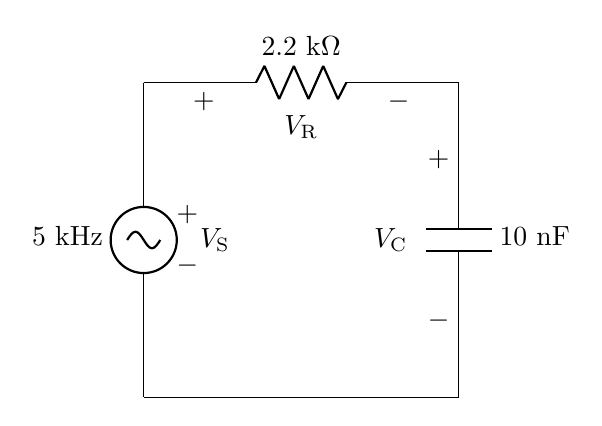
\begin{tikzpicture}
            \draw
                (0,4) to [sV=$V_\text{S}$, l_=$5\text{ kHz}$] (0, 0)
                (0,4) to [R=$2.2\text{ k}\Omega$, v_=$V_\text{R}$] (4, 4)
                to [C=$10\text{ nF}$, v_=$V_\text{C}$] (4, 0)
                to [short, -] (0, 0);
        \end{tikzpicture}
    }
    \subfigure[The Circuit Wiring (including AD2) for $V_C$] {
        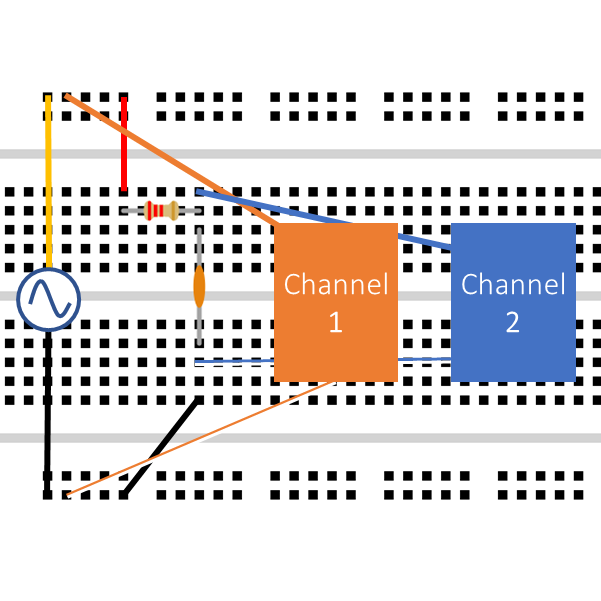
\includegraphics[width=0.3\textwidth]{images/bb1.png}
    }
    \subfigure[The Circuit Wiring (including AD2) for $V_R$] {
        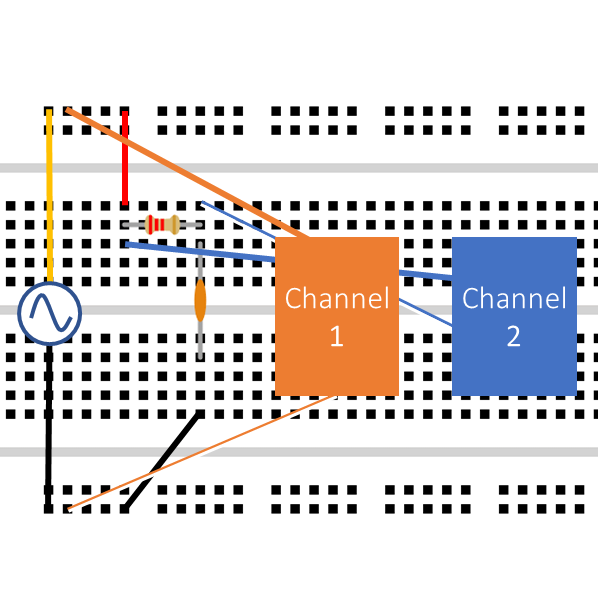
\includegraphics[width=0.3\textwidth]{images/bb2.png}
    }
    \caption{Final Set-Up Utilized}
\end{figure}


The measured resistance of the resistor is \textbf{2.16 k$\Omega$}.

\section{Results}
\begin{table}
    \centering
    \begin{tabular}[H]{|c|P{2cm}|P{1.5cm}|P{2cm}|P{2cm}|P{3cm}|P{3cm}|}
        \hline & Amplitude, $V_o$ (V) & RMS\newline (V) & Measured $\Delta T$ ($\mu$S) & Leading or lagging $V_S$? & Calculated phase angle, $\phi$ (degrees) & Phasor (Amplitude $\angle$ Phase Angle) \\
        \hline $V_\text{S}$ & 3.0216 & 2.1391 & -- & -- & & $3.02\angle 0^\circ{}$ \\
        \hline $V_\text{C}$ & 2.3122 & 1.6349 & 19.518 & lagging & -35.0238 & $2.31\angle -35.0^{\circ}$ \\
        \hline $V_\text{R}$ & 1.7195 & 1.2262 & -28.042 & leading & 50.6946 & $1.72\angle 50.7^{\circ}$ \\
        \hline
    \end{tabular}
\end{table}

\subsection{Why KVL cannot be applied on RMS Voltage}
\begin{tcolorbox}
\begin{align*}
    V_\text{C} + V_\text{R} &= 2.3122 + 1.7195 \\
    &= 4.0317\text{ V} \neq V_\text{S}
\end{align*}

This is likely due to the fact that over the period of the waveform, the Voltage and Current are clearly constantly changing and hence at different points, the impedance is different. Thus, KVL cannot be applied overall since the changing impedances don't add up together to work hand-in-hand in this scenario. KVL applies for instantaneous conditions, whereas the RMS value is in fact the average value.
\end{tcolorbox}

\subsection{Verifying KVL in terms of Phasors}
\begin{tcolorbox}
    \begin{align*}
        V_\text{R} + V_\text{C} &= V_{o, \text{ R}} \angle \phi_R + V_{o, \text{ C}} \angle \phi_C \\
        &= V_{o, \text{ R}} \cos \phi_R  + V_{o, \text{ C}} \cos \phi_C \\
        &= 1.7195 \cos(50.6946) + 2.3122\cos(-35.0238) \\
        &= 2.9827 \cong 3.0126
    \end{align*}

    Thus, KVL does in fact work in the phasor space.
\end{tcolorbox}

\subsection{Phasor Diagram}

\begin{figure}[H]
    \centering
    \begin{tikzpicture}
        \draw[thin,->] (-3.5,0) -- (4.5,0) node[right] {$\Re(x)$};
        \draw[thin,->] (0,-3.5) -- (0,4.5) node[above] {$\Im(x)$};
        
        \foreach \x [count=\xi starting from 0] in {-3,-2,-1,,1,2,3,4}{% ticks
            \draw (\x,2pt) -- (\x,-2pt);
            \draw (2pt,\x) -- (-2pt,\x);
            \ifodd\xi
                \node[anchor=north] at (\x,0) {$\x$};
                \node[anchor=east] at (0,\x) {$\x$};
            \fi
        }
        
        \foreach \point in {(1.89,-1.33),(3.0216,0),(1.09,1.33)}{% points
            \draw (0, 0) -- \point;
            \fill \point circle (2pt);
        }

        \node[anchor=north] at (1.89, -1.33) {$V_\text{C} = 2.31\angle -35.0^\circ{}$}; 
        \node[anchor=south] at (3.0216,0) {$V_\text{S} = 3.02\angle 0^\circ{}$}; 
        \node[anchor=west] at (1.09,1.33) {$V_\text{R} = 1.72\angle 50.7^\circ{}$}; 
    \end{tikzpicture}
    \caption{Phasor Diagram for Activity 1}
\end{figure}


\section{Evaluation}
\subsection{Phasor for $I_\text{S}$}
\begin{tcolorbox}
    \begin{align*}
        \tilde{I_\text{S}} &= \frac{\tilde{V_\text{R}}}{R} \\
        &= \frac{1.72 \angle 50.6946^\circ{}}{2.16 \times 10^3} \\
        &= 0.78182 \angle 50.6946^\circ{} \text{ mA}
    \end{align*}
\end{tcolorbox}

\subsection{$Z_\text{C}$ in terms of $C$}
\begin{tcolorbox}
    \begin{align*}
        Z_\text{C} &= \frac{1}{j\omega C} \\
        &= -\frac{j}{(100\pi \times 10^3)C} \\
        &= -\frac{j}{(31415.92654)C}
    \end{align*}
\end{tcolorbox}

\subsection{Estimate of $C$}
\begin{tcolorbox}
    \begin{align*}
        Z_\text{C} &= \frac{\tilde{V_\text{C}}}{\tilde{I_\text{S}}} \\
        \frac{1}{j(314159.2654)C} &= \frac{2.3122\angle -35.0238^\circ{}}{0.78182 \angle 50.6946^\circ{} \times 10^{-3}} \\
        C &= \frac{0.78182 \angle 50.6946^\circ{} \times 10^{-3}}{31415.92654\times(2.3122\angle 54.9762^\circ{})} \\
        &= 10.73292\text{ nF} \approx \textbf{10.7 nF}
    \end{align*}
\end{tcolorbox}

\subsection{Two Possible Sources of Experimental Errors}
\begin{tcolorbox}
\begin{itemize}
    \item The wires may contain resistance which causes the distribution of phasor voltage to be slightly disproportionate.
    \item The capacitor has non-zero resistance which can also cause said disproportionate distribution of phasor voltage.
\end{itemize}
\end{tcolorbox}

\end{document}
